\chapter{The \g12 Experiment}\label{sec:clas.g12}

The \g12 experiment ran during March - June 2008 with a total of 44 days of good beam time. It collected over 128~TB of raw data that consisted of $26\cdot 10^9$ events, with an integrated luminosity of 68~pb$^{-1}$. A detailed explanation of the \abbr{CLAS} data reconstruction and explanation of the \abbr{DAQ} for \g12 can be found in~\cite{clas.g12.note}. This chapter will briefly overview aspects of the \g12 running conditions and data retrieval found in~\cite{clas.g12.note}. Table~\ref{tab:g12_run_parms} lists the general running conditions of \g12.
\begin{center}
\begin{longtable}{c|c}
\caption[\g12 Running Parameters]{\label{tab:g12_run_parms}Running conditions for \g12}\\

\hline
\endhead
\hline
\endfoot
\hline
\endlastfoot
\hline
Electron Beam Energy & 5.714~GeV \\
Electron Beam Current & 60-65~nA (production) \& 24~nA(single-prong)\\
Electron Beam Polarization & Circular\\
Radiator Material/Density & Au \ / \ 646$\mu\mathrm{g/cm^2}$ \\
Radiator Thickness & $10^{-4} \chi_0$ \\
Radius of Photon collimator & 6.4~mm \\
Photon Beam Energy Range & 1.142-5.425~GeV \\
Target Shell Material & Kapton \\
Target Length/Diameter & 40~cm/4~cm \\
Target Inside Material & $\ell$H$_2$ \\
Target Position & -90~cm from \abbr{CLAS} center \\
Target Polarization & None \\
Torus Magnetic Current & $\frac{1}{2}\mathrm{B}_{max}$ = 1930~A \\
\hline \hline
\end{longtable}
\end{center}
\vspace{20pt}
\newpage
\section{\g12 Data Acquisition and Triggering  }\label{sec:clas.g12.conditions.data}

As described in previous sections, \clas is a detector comprised of several subsystems. Each subsystem in \clas has its own electronics package to monitor its components and collect signals. Discriminators determine whether a signal each each channel a subsystem exceeds a given threshold. In the case of the \abbr{DC} the signal is supplied from the sense wire. For the \abbr{ST}, \abbr{CC}, \abbr{TOF}, \abbr{EC} subsystems, the signal is supplied by converting the current supplied by an anode of a \abbr{PMT} or cluster of \abbr{PMT}'s into a voltage. Each subsystem has a preset voltage threshold. The discriminator compares the signal output of a subsystem to the preset threshold. Signals that exceed the preset threshold are digitized by two types of hardware, Time-to-digital converters (\abbr{TDC}s) and Analog-to-digital converters (\abbr{ADC}s). \abbr{TDC}s report the time at which a signal arrives, while \abbr{ADC}s report a number corresponding to the integral of the signal.

The presence of a signal in a single subsystem does not constitute a physics event. There are a number of unwanted sources that could produce unwanted signals, such as cosmic radiation, electronic noise, Fano noise etc. It is the job of the trigger to determine which sets of signals constituted a physics event. The trigger is a list of signals from various subsystems required for an event to be written out to disk. An item in the trigger list is known as a trigger ``bit''. The \g12 rungroup used a field-programmable gate array (\abbr{FPGA}) as the trigger supervisor. The \abbr{FPGA} allowed for 12 independent trigger configurations to be employed at one time during the running of \g12 as well as the ability to change the trigger configuration during running. The detector subsystems used in the first-level (\abbr{L1}) triggering system of \g12 are the \abbr{TAGR}, \abbr{ST},  \abbr{CC}, \abbr{TOF}, and \abbr{EC}. The \abbr{TOF} and \abbr{ST} are used to identify charged tracks, at the trigger level, by using coincidence of any one \abbr{TOF} hit in a given sector with any one \abbr{ST} hit in the same sector. Also, a coincidence between the \abbr{EC} and \abbr{CC} was included as a lepton trigger. Fig.~\ref{fig:clas.daq.trigsec} depicts the \abbr{L1} trigger configuration for the subsystems mentioned except for the \abbr{TAGR} subsystem. During the \g12 experiment, the interval for a trigger coincidence was 100 ns. All subsystems of \clas except for the \abbr{DC} can acquire signals in a few nanoseconds.
\begin{figure}[h]\begin{center}
\includegraphics[width=0.8\figwidth]{\figures/hall-b/trigger_sector.pdf}
\caption[Trigger logic for one of the six sectors of \abbr{CLAS}]{\label{fig:clas.daq.trigsec}{\coloronline}Trigger logic for one of the six sectors of \abbr{CLAS}. The \abbr{ST$\times$TOF} signal is a coincidence between any of the four start counter \abbr{TDC} signals (numbered from 0 to 3) and any of the 57 \abbr{TOF} \abbr{TDC} signals. The \abbr{ECE}$_\mathrm{inner}$ and \abbr{ECE}$_{\mathrm{total}}$ are the electron-threshold \abbr{EC} signals for the energy deposited in the \emph{inner} layer and in \emph{all} layers. These are combined with a \abbr{CC} signal to produce the \abbr{EC$\times$CC} trigger for this sector. The \abbr{ECP} trigger signal is the photon-threshold \abbr{EC} signal. These trigger signals are discussed further in Sec.~\ref{sec:data.trig}.}
\end{center}\end{figure}

When a first-level trigger requirement is satisfied, a second-level (\abbr{L2}) trigger requirement is sometimes necessary to verify the \abbr{L1} trigger. A \abbr{L2} trigger is usually a software routine unlike the \abbr{L1} trigger which is based on hardware. The \abbr{L2} trigger is typically employed for measurements from the \abbr{DC} and is slower than the \abbr{L1} trigger because it is software based. The software routine does coarse track reconstruction on the \abbr{DC} hits to confirm that the L1 coincidence was caused by particles traveling through \clas rather than unwanted noise.

When a trigger configuration is completely satisfied, the data acquisition system (\abbr{DAQ}) collected the signals and wrote them to magnetic tape for future offline analysis. At the time \g12 was run, the \abbr{DAQ} was capable of running at 8~kHz.

\subsection{\g12 Trigger Configuration} \label{sec:data.trig}
The trigger configuration used in the \g12 running period are listed in Tables~\ref{tab:data.trig.conf.1}, \ref{tab:data.trig.conf.2} and \ref{tab:data.trig.conf.3}. All but one ``bit'' required a (\abbr{ST}$\cdot$\abbr{TOF}) to be present along with other requirements. The (\abbr{ST}$\cdot$\abbr{TOF}) configuration required a track to have coincidence in one sector between any one of the four start counter paddles of that sector, and any one of the 57 time-of-flight paddles in the same sector. Any configuration listed in the Tables~\ref{tab:data.trig.conf.1}, \ref{tab:data.trig.conf.2} and \ref{tab:data.trig.conf.3} with the suffix ``$\times$ N'' after a parenthesis grouped configuration requires that given configuration to have ``N'' coincidences in different sectors. To illustrate this the configuration (\abbr{ST}$\cdot$\abbr{TOF}) requires one coincidence in the same sector, while (\abbr{ST}$\cdot$\abbr{TOF})$\times$ 2 requires two coincidences of (\abbr{ST}$\cdot$\abbr{TOF}) in two different sectors and (\abbr{ST}$\cdot$\abbr{TOF})$\times$ 3 requires three coincidences of (\abbr{ST}$\cdot$\abbr{TOF}) in three different sectors. The hardware and configuration did not allow triggering of two tracks in the same sector because there were only six signals coming from the \abbr{TOF}, one for each sector. 

Another component that can be included into a trigger ``bit'' is ``Master-\abbr{OR},'' (\abbr{MOR}). This component is a signal with the photon tagger. These are defined in Table~\ref{tab:data.trig.mor} and is illustrated with the other components of a ``bit'' in Fig.~\ref{fig:clas.daq.triglogic}.
\begin{figure}[h]\begin{center}
\includegraphics[width=0.8\figwidth]{\figures/hall-b/trigger_logic_w_st.pdf}
\caption[Trigger logic for any of the six sectors of \abbr{CLAS} along with \abbr{MOR} asynchronous logic trigger input]{\label{fig:clas.daq.triglogic}{\coloronline}Trigger logic for any of the six sectors of \abbr{CLAS} along with \abbr{MOR} asynchronous logic trigger input.}
\end{center}\end{figure}

\subsubsection{Lepton Triggering and Neutral Triggering}\label{sec.data.trig.lepton}
In \g12, since the \abbr{CC} was filled with gas, it was possible to include the \abbr{CC} as a component of the trigger. 
There were three trigger ``bits'' used for lepton identification in \g12 as listed in Table~\ref{tab:data.trig.conf.2}. Each ``bit'' used a (\abbr{EC}$\cdot$\abbr{CC}) configuration to identify leptons. The (\abbr{EC}$\cdot$\abbr{CC}) configuration required a coincidence between the electromagnetic calorimeter and the Cherenkov subsystems. This coincidence was established by using the voltage sum of the \abbr{CC} for a sector and the voltage sum of the \abbr{EC} for the same sector and comparing each sum to a preset threshold described in Table~\ref{tab:data.ecccthresh}. The \abbr{EC} voltage sum threshold comparison is done on both the \abbr{EC}$_\mathrm{inner}$ and \abbr{EC}$_{\mathrm{total}}$ which are the \abbr{EC} voltage signals for the energy deposited in the inner layer and in all layers. The labels of photon or electron specified in Table~\ref{tab:data.ecccthresh} are not actual photons or electrons, but were considered a first-order approximation for detection. The particle identification is done at the analysis level. The method for determining the (\abbr{EC}$\cdot$\abbr{CC}) does not allow for multiple lepton triggering in the same sector. Determining multiple leptons in the same sector is done at the analysis level. 

The ``bit 6'' trigger configuration, (\abbr{ST}$\cdot$\abbr{TOF})$\cdot$(\abbr{EC}$\cdot$\abbr{CC}) requires a \abbr{ST} and \abbr{TOF} coincidence previously described in~\ref{sec:data.trig} along with a coincidence between the electromagnetic calorimeter and the Cherenkov subsystems described above. The (\abbr{ST}$\cdot$\abbr{TOF}) configuration of ``bit 6'' did not have to be in the same sector as the (\abbr{EC}$\cdot$\abbr{CC}) configuration of ``bit 6''. The ``bit 11'' trigger configuration, (\abbr{EC}$\cdot$\abbr{CC})$\times$2 requires two coincidences between the electromagnetic calorimeter and the Cherenkov subsystems described above, in two different sectors. 

The ``bit 5'' trigger configuration was also established as a lepton trigger. It required \abbr{EC} hits in two sectors. The ``bit 5'' trigger configuration was also established to analyze physics involving two or more neutral particles accompanied with a charged track, such as exclusive \piz production in which the \piz decays via 2 photons. The method for ``bit 5'' voltage sum comparison is identical to the \abbr{EC} voltage sum of ``bit 6'' and ``bit 11''

It should be noted that none of the lepton triggers required a \abbr{MOR} signal, allowing for physics involving leptons to be measured starting from \g12's lowest tagger detection value of 1.142~GeV.

\begin{table}
\begin{minipage}{\textwidth}
\begin{center}
\begin{singlespacing}

\caption[Trigger Configuration 1]{\label{tab:data.trig.conf.1}Trigger configuration for \g12 runs from 56363 to 56594 and 56608 to 56647. (\abbr{ST}$\cdot$\abbr{TOF})$_{i}$ indicates a trigger-level track defined as a coincidence between a start counter and time-of-flight hit in the \ith\ sector. \abbr{MORA} and \abbr{MORB} represent coincidences with tagger hits within a certain energy range as specified in Table~\ref{tab:data.trig.mor}.}

\begin{tabular}{cccc}

\hline

\multicolumn{4}{c}{\g12 runs 56363--56594, 56608--56647} \\

\hline

bit & definition & L2 multiplicity & prescale \\

\hline

1 & \abbr{MORA}$\cdot$(\abbr{ST}$\cdot$\abbr{TOF})$_{1}\cdot$(\abbr{ST}$\cdot$\abbr{TOF})$_{i\neq 1}$ & -- & 1 \\
2 & \abbr{MORA}$\cdot$(\abbr{ST}$\cdot$\abbr{TOF})$_{2}\cdot$(\abbr{ST}$\cdot$\abbr{TOF})$_{i\neq 2}$ & -- & 1 \\
3 & \abbr{MORA}$\cdot$(\abbr{ST}$\cdot$\abbr{TOF})$_{3}\cdot$(\abbr{ST}$\cdot$\abbr{TOF})$_{i\neq 3}$ & -- & 1 \\
4 & \abbr{MORA}$\cdot$(\abbr{ST}$\cdot$\abbr{TOF})$_{4}\cdot$(\abbr{ST}$\cdot$\abbr{TOF})$_{i\neq 4}$ & -- & 1 \\
5 & \abbr{MORA}$\cdot$(\abbr{ST}$\cdot$\abbr{TOF})$_{5}\cdot$(\abbr{ST}$\cdot$\abbr{TOF})$_{i\neq 5}$ & -- & 1 \\
6 & \abbr{MORA}$\cdot$(\abbr{ST}$\cdot$\abbr{TOF})$_{6}\cdot$(\abbr{ST}$\cdot$\abbr{TOF})$_{i\neq 6}$ & -- & 1 \\
7 & \abbr{ST}$\cdot$\abbr{TOF} & -- & 1 \\
8 & \abbr{MORA}$\cdot$(\abbr{ST}$\cdot$\abbr{TOF})$\times$2 & -- & 1 \\
11\footnote{bit 11 and \abbr{MORB} were included in the trigger starting with run 56519.} & \abbr{MORB}$\cdot$(\abbr{ST}$\cdot$\abbr{TOF})$\times$2 & -- & 1 \\
12 & (\abbr{ST}$\cdot$\abbr{TOF})$\times$3 & -- & 1 \\

\hline \hline

\end{tabular}

\end{singlespacing}
\end{center}
\end{minipage}
\end{table}
\vspace{20pt}
 % label: tab:data.trig.conf.1

\input{tables/trigger_config_2} % label: tab:data.trig.conf.2

\input{tables/trigger_config_3} % label: tab:data.trig.conf.3

\input{tables/trigger_mor.tex} % label:  tab:data.trig.mor

\begin{table}
\begin{center}
\begin{singlespacing}

\caption[\abbr{EC} and \abbr{CC} Trigger Thresholds]{\label{tab:data.ecccthresh}Threshold values for the electromagnetic calorimeter (\abbr{EC}) and Cherenkov counter (\abbr{CC}) during the \g12 running period. \abbr{EC} thresholds are shown as \emph{inner}/\emph{total}, and \abbr{CC} thresholds are shown as \emph{left}/\emph{right}.\vspace{0.75mm}}

\begin{tabular}{cc|c}
\hline

\multicolumn{2}{c|}{\abbr{EC}} & \abbr{CC} \\

\emph{``photon"} & \emph{``electron"} \\


\hline

50/100~mV & 60/80~mV & 20/20~mV \\
150/300~MeV & 180/240~MeV & $\sim$0.4~photo-electrons \\

\hline \hline

\end{tabular}

\end{singlespacing}
\end{center}
\end{table}
\vspace{20pt} % label: tab:data.ecccthresh

\FloatBarrier

\section{\g12 Run Summary}\label{sec:clas.g12.runs}

The \g12 experiment was divided into 626 production runs, 37 single-prong runs, 13 special calibration runs and numerous diagnostic runs which were not recorded. Each run consisted of approximately 50 million triggered events. Table~\ref{tab:data.cook.prodruns} contains a list of the runs that had at least 1M triggers and were reconstructed successfully, along with the beam current for these runs. If a run did not have at least 1M triggered events or if the run was corrupt, the run was discarded.
\input{tables/g12_prod_runs}
%

The single-prong data runs were incorporated into the \g12 running upon approval of proposal \cite{clas.proposal.pion}. This data was obtained using a trigger requirement of a single track hit in a sector of \abbr{CLAS}. In order to properly trigger a single hit in the \abbr{DC} a lower current of 24~nA was used. This portion of the data has yet to be examined for any physics purpose, however the data had been preliminarily reconstructed by the author of this document. It was determined that timing calibrations must be redone for this specific data set. The amount of data that can be analyzed in these 37 runs is approximately equal to 60~\% the amount of data in the higher current production runs. See Table~\ref{tab:data.cook.singlesecruns}.
\begin{table}
\begin{minipage}{\textwidth}
\begin{center}
\begin{singlespacing}

\caption[Single-prong Run List]{\label{tab:data.cook.singlesecruns}A list of the single-prong runs using the trigger configuration described in Table~\ref{tab:data.trig.conf.3}.\vspace{0.75mm}}

\begin{tabular}{lr|lr}

\hline
run & current (nA) & run & current (nA) \\
\hline

56476 & 24 & 56910 & 35 \\
56502 & 24 & 56911 & 30 \\
56520 & 24 & 56912 & 25 \\
56544 & 24 & 56913 & 24 \\
56559 & 24 & 56933-56934 & 24 \\
56585 & 24 & 56981-56983 & 24 \\
%56619 & 24 & 56985\footnotemark{foot:no_l2} & 15 \\ 
56619 & 24 & 56985 & 15 \\
56637 & 24 & 56986 & 15 \\
56663-56664 & 24 & 56989 & 24 \\
56697 & 24 & 57028 & 24 \\
56725 & 24 & 57061 & 24 \\
56747 & 24 & 57094 & 24 \\
56769 & 24 & 57129 & 24 \\
56804 & 24 & 57155-57156 & 24 \\
56835 & 24 & 57237-57238 & 24 \\
56869 & 5 \\

\hline \hline

\end{tabular}

\end{singlespacing}
\end{center}
\end{minipage}
\end{table}
\vspace{20pt} % 

Listed in Table~\ref{tab:data.calibruns} are several special calibration runs. These runs consist of normalization, zero-field, and empty-target data runs. The normalization runs were used to calibrate the tagger for the measurement of the total photon flux and consistency of the left and right \abbr{TDC} signals of the tagger. The zero-field data was taken with the main torus magnet off. This was done to account for the position and orientation of the drift-chambers in the reconstruction. The empty target runs were used to investigate the contributions of the target wall to the data sample.
\begin{center}
\begin{singlespacing}
\begin{longtable}{ccl}
\caption[\g12 Special Run List]{\label{tab:data.calibruns}List of special calibration runs done during the \g12 experiment.} \\

\hline
run & current (nA) & description \\
\hline
\endfirsthead

\multicolumn{3}{l}{\scriptsize continued from previous page.} \\
\hline
run & current (nA) & description \\
\hline
\endhead

\hline
\multicolumn{3}{r}{\scriptsize continued on next page.} \\
\endfoot

\hline \hline
\endlastfoot

56397 & 0.05 & normalization \\
56475 & 10 & zero-field \\
56511 & 0.05 & normalization \\
56512 & 0.05 & normalization \\
56584 & 0.05 & normalization \\
56682 & 0.05 & normalization \\
56790 & 0.05 & normalization \\
56931 & 0.05 & normalization \\
56947 & 0.05 & normalization \\
57169 & 0.05 & normalization \\
57239 & 24 & empty-target, single-sector \\
57241 & 80 & empty-target, production \\
57248 & 0.05 & normalization

\end{longtable}
\end{singlespacing}
\end{center}
\vspace{20pt} 

%
\FloatBarrier
\newpage
\section{Raw Data Reconstruction}\label{sec:data.cook}

The process of reconstructing tracks and their subsequent particle identification from raw data is referred to as ``cooking'' and was done by the program \texttt{a1c}\label{abbr:a1c} for \g12. ``Cooking'' is when the information recorded from the various detector subsystems is converted into a form suitable for physics analysis. During cooking, each detector subsystem was calibrated. The ``cooking'' of the \g12 dataset was performed by John Theodore Goetz and is fully documented in~\cite{clas.g12.note} and~\cite{goetz}.

The ``cooking'' process performed by \texttt{a1c} is outlined in Fig.~\ref{fig:data.cook.flowchart}. Initial calibrations are done for each subsystem in each sector the process begins with ``hit-based'' tracking in the \abbr{DC}. ``Hit-based'' tracking requires only the positions of wires registering a hit in a given sector. Adjacent hits in each superlayer are assembled into clusters, and then these clusters are linked in each region to produce track segments. Refer to Fig.~\ref{fig:clas.dc.drift} for an illustration of a track segment. Track segments are linked over the three regions to produce full hit-based trajectories. See Fig~\ref{fig:data.cook.flowchart.hitbased} for a pictorial description of ``hit-based'' tracking. There was an overall failure of events that should have passed ``hit-based'' tracking but failed. This will be discussed fully in Sec.~\ref{sec:analysis.accept.verify}.
%, but can be seen in Fig.~\ref{sec:clas.st.eff} as an overall inefficiency of 3.75\%.

\begin{figure}\begin{center}
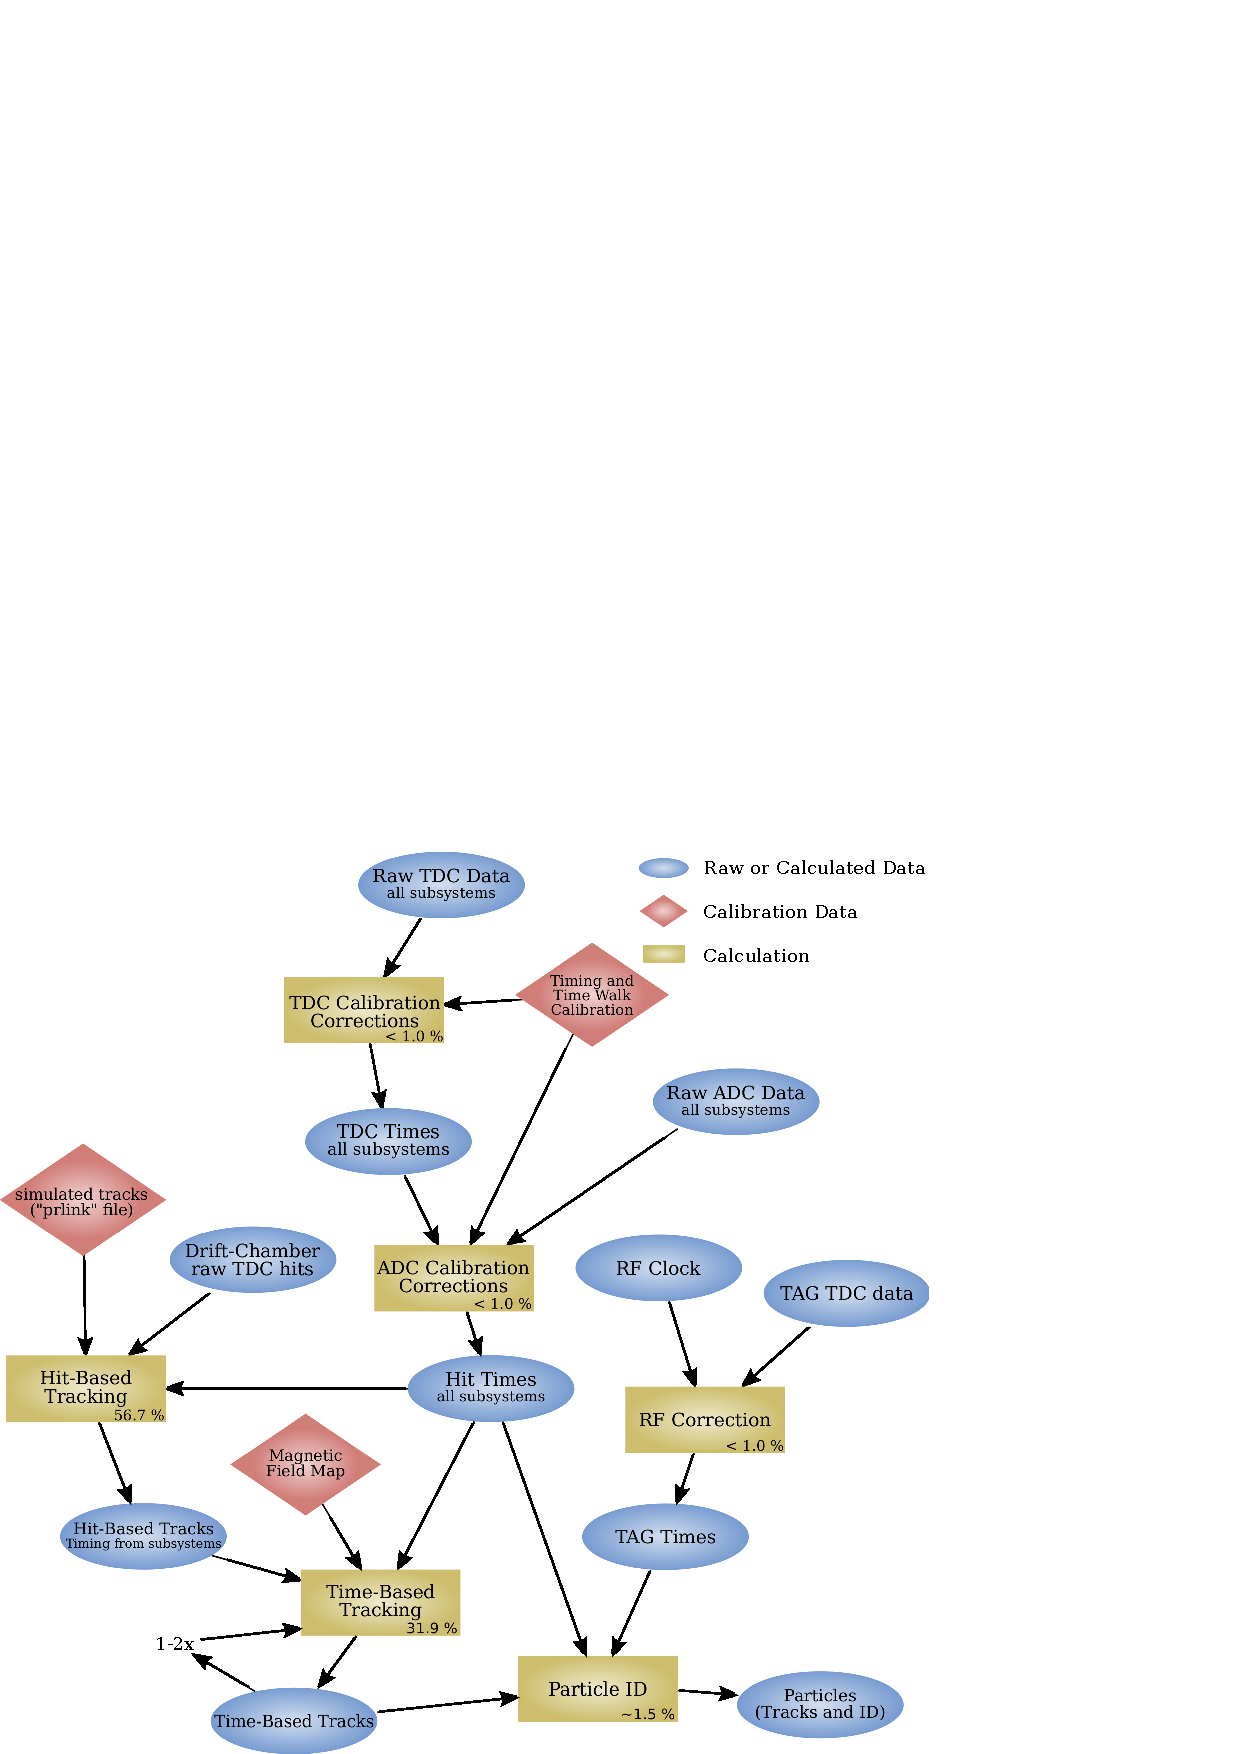
\includegraphics[width=0.92\columnwidth]{\figures/reconstruction/clas6_cooking_diagram_color.pdf}
\caption[Flow chart of the reconstruction process from raw data to identified tracks with momentum]{\label{fig:data.cook.flowchart}Flow chart of the reconstruction process from raw data to identified tracks with momentum. ``Subsystems'' refers to the \abbr{ST}, \abbr{CC}, \abbr{TOF} and the \abbr{EC} detectors. Percentages shown indicate the relative time taken to do the calculations.}
\end{center}\end{figure}

\begin{figure}\begin{center}
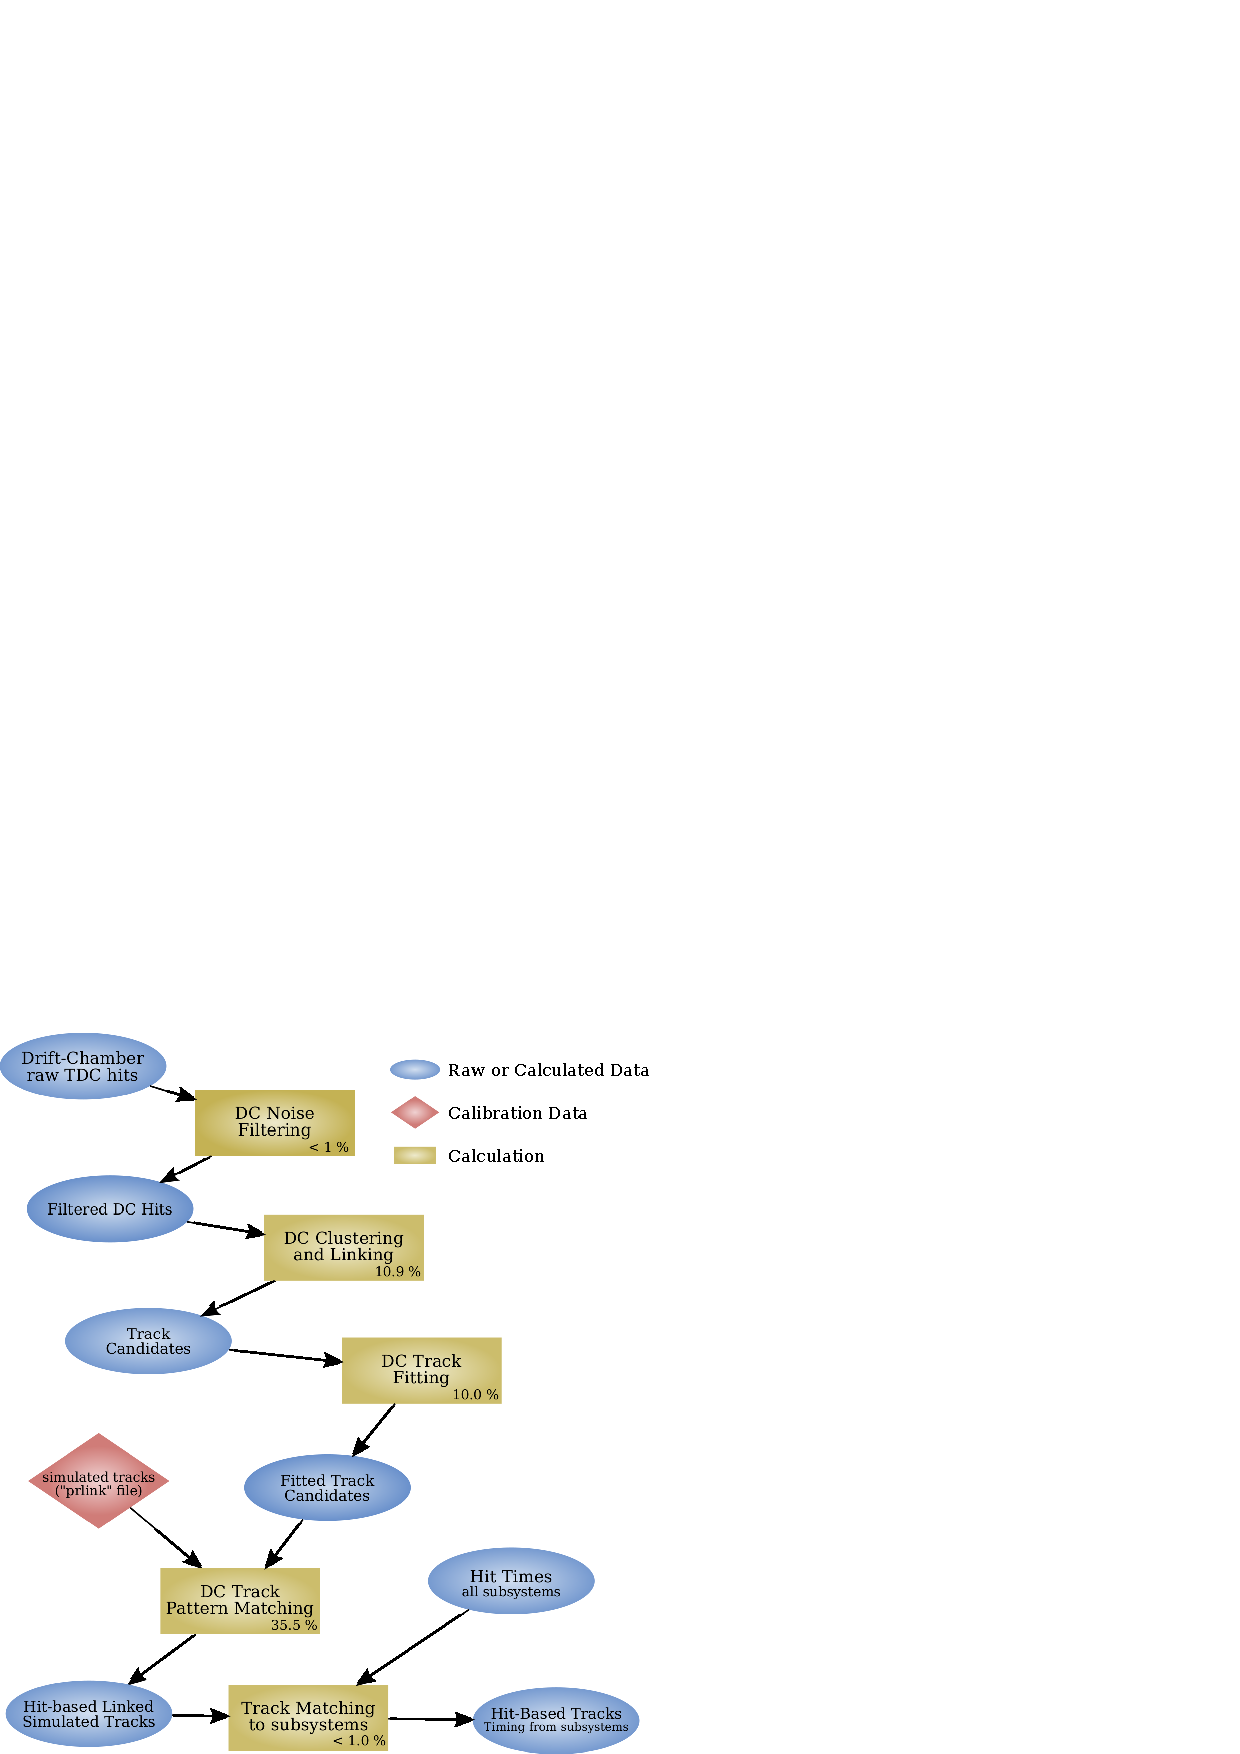
\includegraphics[width=0.7\columnwidth]{\figures/reconstruction/clas6_hitbasedtracking_diagram_color.pdf}
\caption[Flow chart of the hit-based tracking part of the reconstruction]{\label{fig:data.cook.flowchart.hitbased}Flow chart of the hit-based tracking part of the reconstruction shown in Fig.\ref{fig:data.cook.flowchart}. ``Subsystems'' refers to the \abbr{ST}, \abbr{CC}, \abbr{TOF} and the \abbr{EC} detectors. Percentages shown indicate the relative time taken to do the calculations with respect to the full reconstruction.}
\end{center}\end{figure}


After ``hit-based'' tracking is performed, ``time-based'' tracking is performed on the hits obtained from ``hit-based'' track to the appropriate \abbr{TOF} panel. This is done to eliminate noise hits or whole clusters that are not associated with physical tracks. If a hit from ``hit-based'' tracking is found to match a \abbr{TOF} panel, the time measurement from the \abbr{TOF} panel is used to set an upper limit to the time of the drift-chamber hits. With this upper limit known, the \abbr{DC} hits associated with the track are checked individually, where each hit is required to be in increasing time order as the track moves away from the target, any hits or whole clusters not satisfying this requirement are removed. After the removal of the initial bad hits, the track is refit using the remaining hits and the process of removing bad hits is repeated up to two more times to further refine momentum measurements, as well as the measurement of the event vertex, which is determined by the distance of closest approach of the track to the beamline. When the processes of ``time-based'' tracking is finished, all other subsystem information is then added to the tracks properties list. See Fig~\ref{fig:data.cook.flowchart.timebased} for a pictorial description of ``time-based'' tracking. 

During the initial stages of ``time-based'' tracking, a \abbr{ST} signal must be present. This will be discussed in Sec.~\ref{sec:analysis.accept.verify}.  If the track failed due to this error, it usually passed ``time-based'' on the second or third pass of the ``time-based'' tracking if another particle passed ``time-based'' during the initial pass. The average inefficiency for three track events for data was $<0.01$\%
% that there was a random bug in the processing of the \abbr{TDC} element information of \abbr{ST} (\abbr{STN0}) and the \abbr{ADC} element information of \abbr{ST} (\abbr{STN1}) raw data banks. The bug miscalculated the tracks sector exiting the \abbr{ST} even as the hit element of the \abbr{ST} matched that to the track in the \abbr{DC}. This inefficiency can be seen in Fig.~\ref{sec:clas.st.eff}. If the track failed due to this error, it usually passed ``time-based'' on the second or third pass of the ``time-based'' tracking if another particle passed ``time-based'' during the initial pass. The average inefficiency for three track events for data was 0.0125\%

The process of ``cooking'' was performed for Monte-Carlo data for the purpose of verifying the simulation package and the presence of this error and the ``hit-based'' inefficiency is discussed in Sec.~\ref{sec:analysis.accept.verify}.

\begin{figure}\begin{center}
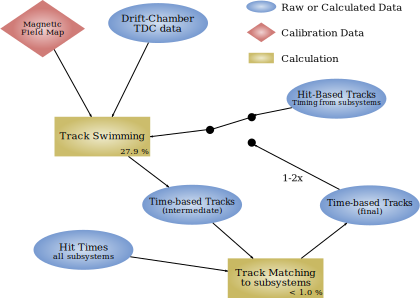
\includegraphics[width=0.8\columnwidth]{\figures/reconstruction/clas6_timebasedtracking_diagram_color.pdf}
\caption[Flow chart of the time-based tracking part of the reconstruction]{\label{fig:data.cook.flowchart.timebased}Flow chart of the time-based tracking part of the reconstruction shown in Fig.\ref{fig:data.cook.flowchart}. ``Subsystems'' refers to the \abbr{ST}, \abbr{CC}, \abbr{TOF} and the \abbr{EC} detectors. The switch indicates that hit-based tracks are input into the swimming calculation, after which the time-based tracks are used creating a feedback loop. Percentages shown indicate the relative time taken to do the calculations with respect to the full reconstruction.}
\end{center}\end{figure}




%The tagger energy was calibrated using the exclusive reaction:
%\begin{align}\label{rxn:excl_ppippim}
%    \mathrm{\gamma p \rightarrow p \pi^+ \pi^-}
%\end{align}
%where the exclusivity was determined via missing momentum and missing mass cuts using the energy of the tagger hit associated with the event. The photon energy was then adjusted by taking the total energy of the $\mathrm{p \pi^+ \pi^-}$ system using the equation:
%\begin{align}\label{eqn:ebeam_ppippim}
%    E_\mathrm{beam, corrected} = E_\p + E_{\mathrm{\pi^+}} + E_{\mathrm{\pi^-}} - m_\p,   
%\end{align}
%where $E_\p$, $E_{\mathrm{\pi^+}}$ and $E_{\mathrm{\pi^-}}$ are the energies of the outgoing particles, and $m_\p$ is the proton (target) mass. The average of at least 10k events per \emph{logical} tagger energy paddle (see Sec.~\ref{sec:clas.tagr}) was used for this correction and the results as a function of the beam energy is shown in Fig.~\ref{fig:data.calib.tag_energy}. The inherent resolution of the tagger paddles for \g12 was approximately 5.6~MeV.
%
%Results from the tagger energy calibration were used to calculate corrections to the momenta of the tracks, the energy corrections were subsequently recalculated. This iterative process was employed several times until the values obtained for both corrections converged. The energy difference between $E_\mathrm{beam, corrected}$ in Eq.~\ref{eqn:ebeam_ppippim} and the energy reported by the tagger is shown in Fig.~\ref{fig:data.calib.ediff_ppippim}.
%
%The resolution of the tagger time is approximately 130~ps as shown in Fig.~\ref{fig:data.calib.dttag_ppippim} and this value is used to identify the \abbr{RF} beam-bucket associated with the event. The \abbr{RF} provides the best timing resolution, on the order of a few picoseconds, in \abbr{CLAS} and it is used to calibrate the other systems as described in the sections below.

\section{Particle Identification}\label{sec:data.pid}

The final procedure is to assign the track a particle mass ($m$). In Sec.~\ref{sec:clas.tof} Eqs.~\ref{eq:beta.cal} and~\ref{eq:mass.cal} explain how the mass of a particle is determined. Fig.~\ref{fig:data.pid} depicts a 2-dimensional plot of the quantities used to determine the particle mass. Once the mass has been determined, particle identification \abbr{PID} is determined by the following criteria;
%Figure~\ref{fig:data.pid} depicts a plot of the quantities used to determine the particles mass,
\begin{align}\label{list:pid}
\abbr{PID} =
\begin{cases}
\pi^{\pm}, & \mathrm{if} \  m  <  0.3~\mathrm{GeV} \ \mathrm{and} \  q  \pm \\
K^{\pm}, &  \mathrm{if} \ 0.35 < m  <  0.35~\mathrm{GeV} \ \mathrm{and} \  q  \pm  \\
p^{\pm}, & \mathrm{if \ 0.8 \ < \ }m \mathrm{\ < \ 1.2 \ GeV \  and \  q  \pm} \\
d, & \mathrm{if \ 1.75 \ < \  }m  \mathrm{\ < \ 2.2 \ GeV } \\
\end{cases}
\end{align}
The events which had particles falling within the undefined regions of the cuts listed in Eq.~\ref{list:pid} were deemed ambiguous events and were given the \abbr{PID} of \emph{``unknown''}. For the analysis of this work, \emph{``unknown''} were used and is described in Sec.~\ref{sec:analysis}

Since tracking began after the particle had already traversed through the target and \abbr{ST}, the measured momentum determination was decreased by the ``energy-loss'' the particle underwent before entering the Region 1 \abbr{DC}. These effects were taken into account as part of the ``energy-loss'' correction during the analysis phase as discussed in Sec.~\ref{sec:analysis.corrections.eloss}.  Once particle identification is completed on the reconstruction level, all relevant information about the particle is collected into the event of occurrence and this information is written in \abbr{BOS} format. There are multiple methods for analyzing \abbr{BOS} format, the chapter~\ref{sec:analysis} will discuss the method used in this analysis. 
%
\begin{figure}\begin{center}
\includegraphics[width=0.9\columnwidth,height=\hfigheight]{\figures/hall-b/g12_pid.pdf}
\caption[$\beta$ vs. mometum(p)$\times$charge(q) for run 56855]{\label{fig:data.pid} $\beta$ vs. mometum(p)$\times$charge(q) for run 56855. This plot is a graphical representation of how particle ID assignments are made in CLAS reconstruction. The ``ribs" seen represent tracks that were ``out-of-time" with a incident photon. Image Source:~\cite{bookwalter}}
\end{center}\end{figure}
